\section{Explainable AI 2}
Desirable algotithmic features:
\begin{itemize}
    \item Efficient
    \item Obeys mathematical axioms
    \item Model agnostic
    \item Requires single instance
    \item Can solve XOR
    \item Robust to hyperparameters
    \item Data agnostic
\end{itemize}
\subsubsection{Occlusion (Sliding Windows)}
Problems?:
\begin{itemize}
    \item Size of Occluded region
    \item Lenght of side
    \item Return different
    \item Explanations
    \item XOR
    \item Basline?
\end{itemize}
Features:
\begin{itemize}
    \item Model agnostic
    \item Requires single instance
\end{itemize}
Problems:
\begin{itemize}
    \item No saliency fine grained heatmap
\end{itemize}

\subsubsection{Occlusion (Adaptive Occlusion)}
\begin{figure}[!h]
    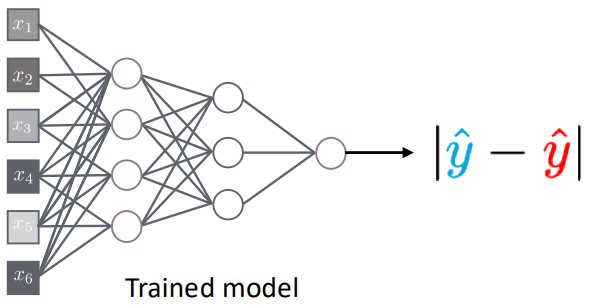
\includegraphics[width = 0.7 \columnwidth]{figures/XAI2/AdaptiveOcclusionNetwork.png}
\end{figure}
\begin{figure}[!h]
    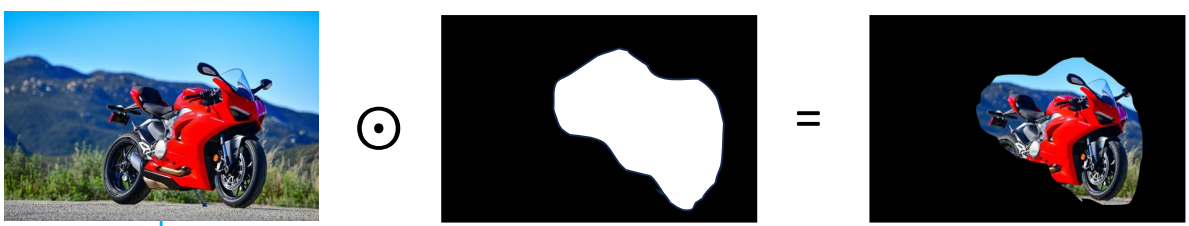
\includegraphics[width =  \columnwidth]{figures/XAI2/AdaptiveOcclusionPictures.png}
\end{figure}

Attemps to minimize the occluded area while maintaining the same prediction outcome as the original.
The goal is to find the smallest and most informative regions that are crucial for the model's decision.
It's an advanced, model-agnostic method that iteratively refines the occluded areas.
\begin{itemize}
    \item \(\hat{y}_{blue}\) is raw picture.
    \item \(\hat{y}_{red}\) is after occlusion.
\end{itemize}
\[
\mathcal{L} = |\hat{y}_{blue}-\hat{y}_{red}| + \alpha \sum_{i \neq 0}|m_i|
\]
Constraints:
\begin{enumerate}
    \item Output predictions must be similar
    \item Must find the most compact area (less pixels better)
\end{enumerate}
Features:
\begin{itemize}
    \item Model agnostic
    \item Requires single instance
\end{itemize}
Problems:
\begin{itemize}
    \item Functions more like image segementation technique
    \item No saliency fine grained heatmap
\end{itemize}


\subsection{Occlusion (Randomized)}
\begin{figure}[!h]
    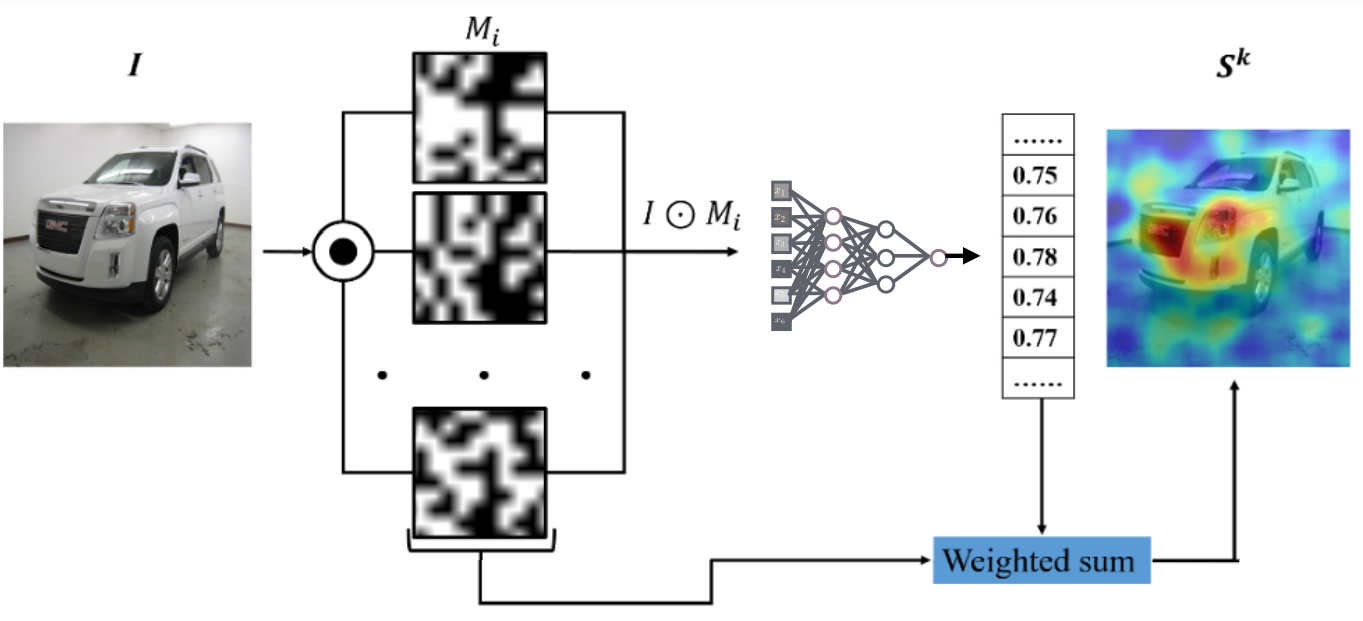
\includegraphics[width =  \columnwidth]{figures/XAI2/RandomizedOcclusion.png}
\end{figure}
Adaptive occlusion only is more like image segementation, does not indicate fine grained decision detail.
Randomized approaches allow us to construct heatmaps.
\begin{enumerate}
    \item Pointwise multiplication of instance \(I\) with mask \(M_i\)
    \item Forward pass through model
    \item Model score is calculated
    \item Repeat for n random masks
    \item Normalize scores
    \item Weigh each mask with normalized score
    \item Sum weighted masks
\end{enumerate}
Problems:
\begin{itemize}
    \item Requires forward passes to minimize the noise
    \item So high computational complexity
    \item Has saliency fine grained heatmap
\end{itemize}
Features:
\begin{itemize}
    \item Model agnostic
    \item Requires single instance
    \item Can solve XOR
    \item Robust to hyperparameters
\end{itemize}

\subsection{Class Activation Mapping(Convolutional Neural Network)}
\begin{figure}[!h]
    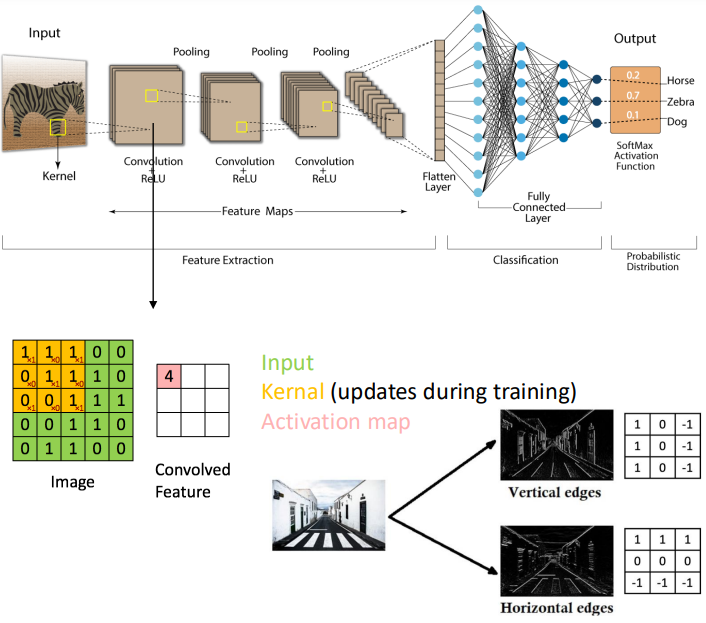
\includegraphics[width =  \columnwidth]{figures/XAI2/CAMCNN.png}
\end{figure}
Convolutional layers from a hierarchy of abstractions.
\begin{itemize}
    \item First maps identify edges
    \item Last maps identify complex patterns
\end{itemize}
\subsubsection{Activation Mapping}
Activation maps are in image/pixel space.
Important to realize, the feature activation maps light up if a pattern is present in the input image!
Each map is searching for a different high level pattern.

\subsection{Class Activation Mapping (CAM)}
\begin{figure}[!h]
    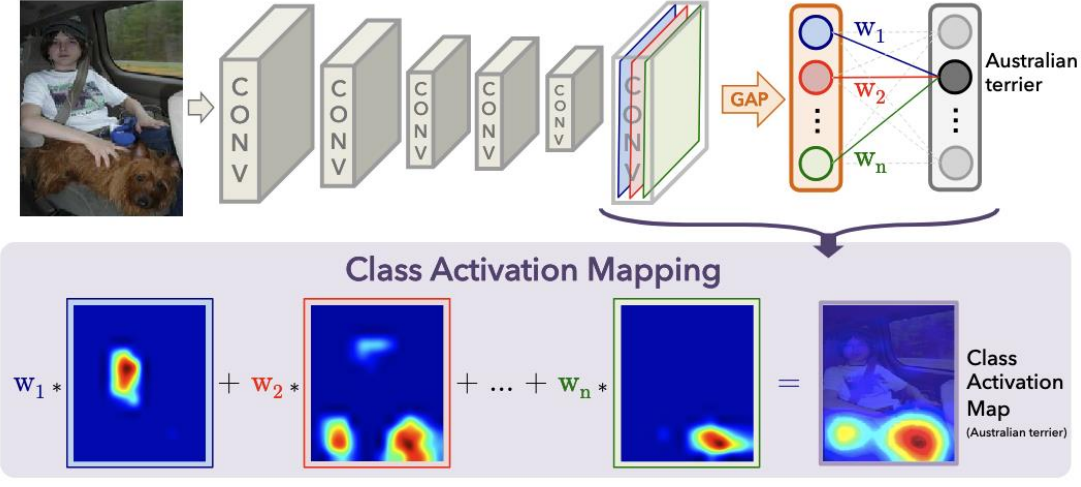
\includegraphics[width =  \columnwidth]{figures/XAI2/CAM.png}
\end{figure}
\begin{enumerate}
    \item Architecture dependant
    \item Global average pooling layer
    \item Straight into SoftMax function for class prediction
    \item Results in a linear (white box) model where the weights express the relative importance of each feature identifies.
\end{enumerate}
Global average pooling
\[
\sigma(z)_i = \frac{e^{z_i}}{\sum_{j = 1}^{K}e^{z_i}} \qquad M^c = ReLU\left(\sum_{k}w_k^c A^k\right)
\]
Features:
\begin{itemize}
    \item Efficient
    \item Requires single instance
    \item Can solve XOR
\end{itemize}

Problems:
\begin{itemize}
    \item Extremly architecturally dependent
\end{itemize}
\subsection{Grad-CAM}
Feature map weights calculated as average effect each pixel has on the output if slightly pertubed:
\[
\alpha_k^c = \frac{1}{Z}\sum_{i} \frac{\partial y^c}{\partial A_i^k}
\]
Heatmap generated as weighted sum of feature maps ReLU is used to show positive discriminant area:
\[
M^c = ReLU\left(\sum_{k}\alpha_k^c A^k\right)
\]
Upscale map to resolution of the original image. This means size of the final feature layer is critical.
\begin{figure}[!h]
    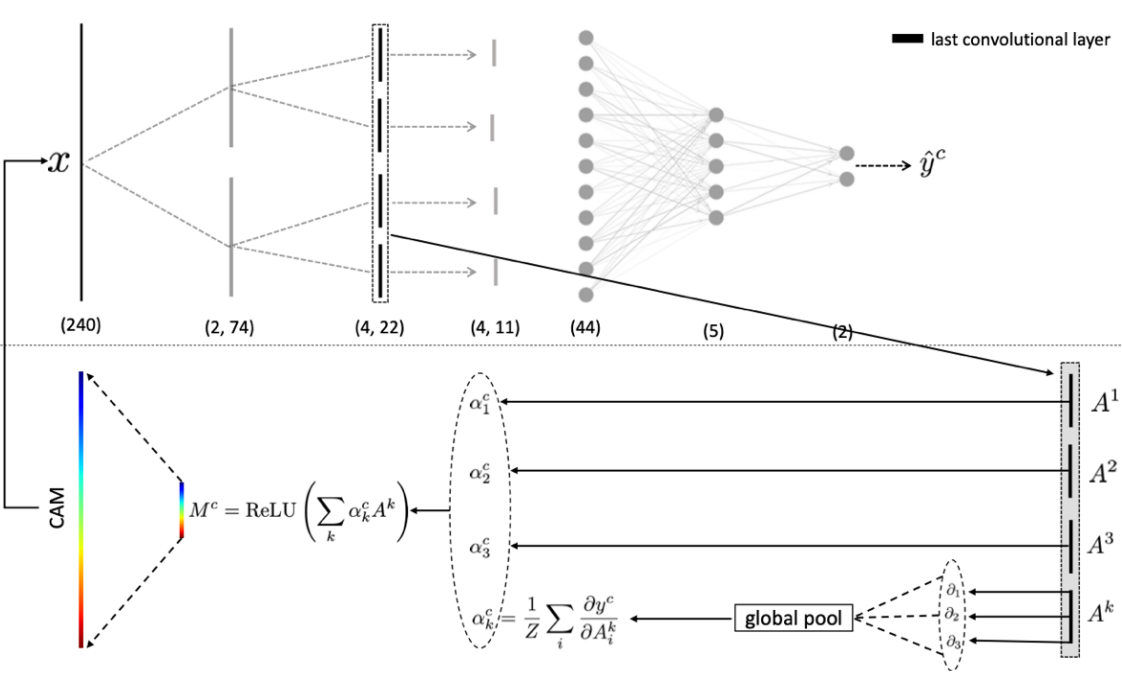
\includegraphics[width =  \columnwidth]{figures/XAI2/GRADCAM.png}
\end{figure}
\begin{enumerate}
    \item Frees up architecture constraints
    \item Don't have to compromise accuracy as final conv layer can go into any function, not just SoftMax
    \item Final feature map resolution dictates the graduality of the explanation
    \item Tension between high level semantics and explanatory resolution
    \item Cannot compare the intensity of final heatmaps between different instances
    \item Still requires CNN
\end{enumerate}
Features:
\begin{itemize}
    \item Efficient
    \item Requires single instance
    \item Can solve XOR
\end{itemize}
Problems:
\begin{itemize}
    \item Semantically meaningfull features but poor resolution
\end{itemize}

\subsection{Guided Grad-CAM}
\begin{figure}[!h]
    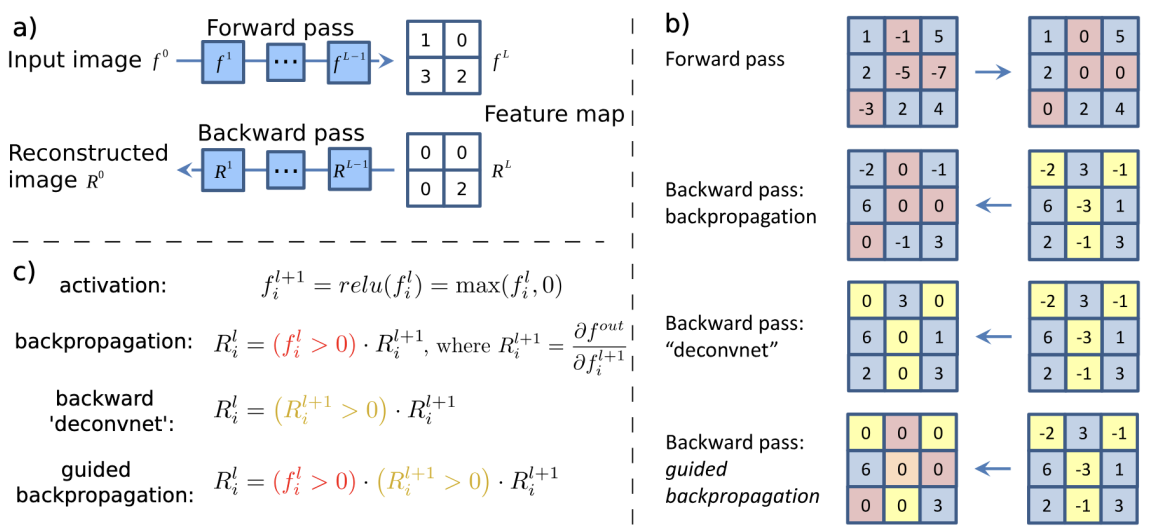
\includegraphics[width =  \columnwidth]{figures/XAI2/GuidedGRADCAM.png}
\end{figure}
\begin{itemize}
    \item Guided Backpropagation \(\rightarrow\) High resolution, basic features
    \item Grad-CAM \(\rightarrow\) Low resolution, abstract semantic features
    \item Guided Grad-CAM \(\rightarrow\) High resolution, semantically rich features
\end{itemize}

\subsection{Gradient X Input}
\begin{itemize}
    \item Simple fast method
    \item Saliency method
    \item Gradient method
    \item Sensitivity of prediction on the input
    \item Multiply the gradient by its features value to scale the sensitivity and provide both importance and direction
\end{itemize}
\(x_i\): Word, Feature, Pixel value

\(f(x)\): LLM, CNN, etc.
\[
M_i = x_i \cdot \frac{\partial f(x)}{\partial x_i}
\]
Features:
\begin{itemize}
    \item Efficient
    \item Model agnostic
    \item Requires single instance
    \item Can solve XOR
    \item Robust to hyperparameters
    \item Data agnostic
\end{itemize}
Looks amazing, why do we need something else:
\begin{itemize}
    \item Each pixel value is calculated independently of its neighbours
    \item In deep networks vanishing gradients compromise the interpretability of the shallow layers
    \item Sensitivity to pixel values introduce bias:
    It is important to multiply the gradient with the input values however this can bias the result in an image where an object is dark but important, Gradient X Input might minimize its importance because of its low pixel values, even if model output would change significantly if that region were alterd.
    \item Not a human level contextual explanation
\end{itemize}
\subsection{Integrated Gradients}
Intuition why we require a different gradient method:
Once a model is confident of its prediction, changing a few pixel values is likely to not change the models prediction.
This is due to how contextually dependant (correlated) image data is.
When a model learns how a value of a specific pixel affects the model's prediction, the gradient for that pixel will become smaller and smaller until it is eventually zero. This is called saturation.

We therefore require a trick that allows us to access the gradient information of each pixel when the model is more sensitive to its charge.

\[
\phi_i^{IG}(f,x,x') = (x_i - x_i')\int_{\alpha = 0}^{1} \frac{\delta f(x' + \alpha(x - x'))}{\delta x_i}d\alpha
\]
Integrate along a path in image space.

\(\alpha\): Linearly interpolate between baseline and target

\(\phi_i^{IG}(f,x,x')\): Attribution for a single pixel \((i )\) given a function and a baseline

\(f\): NN 

\(x\): Target

\(x'\): Baseline 
